\section{Resultados}

O F1 macro de teste atribui o mesmo peso a cada uma das cinco classes. Em cada treino, a época avaliada no teste foi selecionada pelo maior F1 macro de validação.

Das 22 configurações previstas, 20 aguardam entrega de métricas.

A ResNet-18 com inicialização aleatória obteve F1 macro de 0,608 com aumento de dados e de 0,717 sem aumento.

O maior valor ocorreu no caso nenhum, com diferença de 0,109 entre as configurações.

\begin{table}[t]\centering\caption{Desempenho por configuração. Traços indicam resultados pendentes.}
\label{tab:gabriel}\footnotesize\begin{tabular}{llrrr}\hline
Rede & Caso & F1 val. & Acur. teste & F1 teste \\ \hline
ResNet-18 & 1+2 & --- & --- & --- \\
ResNet-18 & 1 & --- & --- & --- \\
ResNet-18 & 2 & --- & --- & --- \\
ResNet-18 & nenhum & --- & --- & --- \\
ResNet-50 & 1+2 & --- & --- & --- \\
ResNet-50 & 1 & --- & --- & --- \\
ResNet-50 & 2 & --- & --- & --- \\
ResNet-50 & nenhum & --- & --- & --- \\
EfficientNet-B0 & 1+2 & --- & --- & --- \\
EfficientNet-B0 & 1 & --- & --- & --- \\
EfficientNet-B0 & 2 & --- & --- & --- \\
EfficientNet-B0 & nenhum & --- & --- & --- \\
MobileNetV3-Large & 1+2 & --- & --- & --- \\
MobileNetV3-Large & 1 & --- & --- & --- \\
MobileNetV3-Large & 2 & --- & --- & --- \\
MobileNetV3-Large & nenhum & --- & --- & --- \\
ConvNeXt-Tiny & 1+2 & --- & --- & --- \\
ConvNeXt-Tiny & 1 & --- & --- & --- \\
ConvNeXt-Tiny & 2 & --- & --- & --- \\
ConvNeXt-Tiny & nenhum & --- & --- & --- \\
ResNet-18 do zero & 1 & 0,667 & 0,705 & 0,608 \\
ResNet-18 do zero & nenhum & 0,772 & 0,817 & 0,717 \\
\hline\end{tabular}\end{table}


\begin{figure}[t]\centering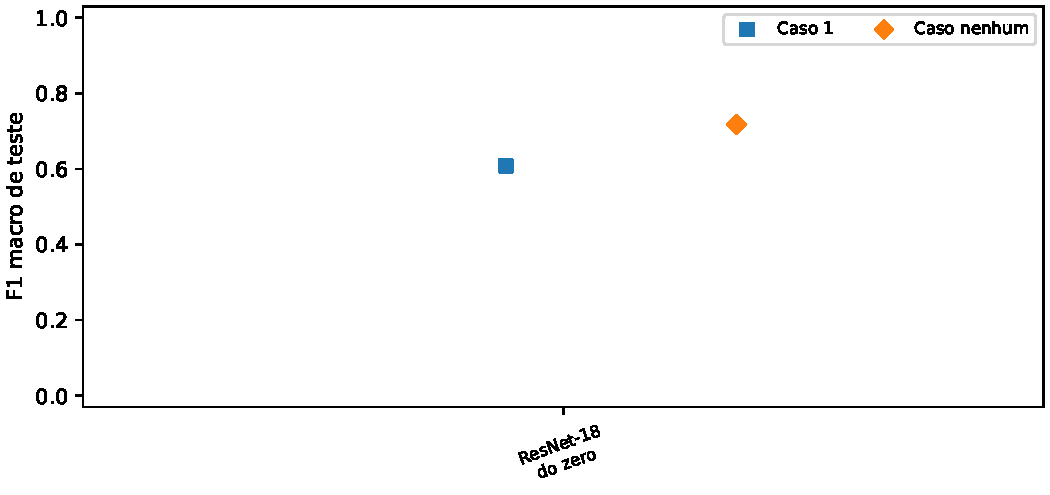
\includegraphics[width=\columnwidth]{artigo/gabriel/gerado/f1_por_rede.pdf}\caption{F1 macro no teste por rede e configuração.}\end{figure}

\section{Conclusão}

A comparação global depende da consolidação dos resultados pendentes.

A comparação de inicializações também incorpora as taxas de aprendizado da base previstas em cada protocolo. A avaliação usa uma divisão única e uma semente por configuração. Na divisão local, 238 conteúdos de fotos originais, identificados por SHA-256, ocorrem tanto no treino quanto no teste. Entre as 1.257 entradas finais de teste, 19 são idênticas, byte a byte, a entradas de treino. Essa sobreposição e a proximidade entre capturas limitam a interpretação dos escores como estimativas para imagens inéditas.
